\documentclass{sig-alternate}

\usepackage{packages}

\newcommand{\sharedaffiliation}[0]{\end{tabular}\\\begin{tabular}{c}}

\title{Bug Isolation via Remote Program Sampling
  %%
  \thanks{This research was supported in part by NASA Grant
    No. NAG2-1210; NSF Grant Nos. EIA-9802069, CCR-0085949,
    ACI-9619020, and IIS-9988642; DOE Prime Contract No. W-7405-ENG-48
    through Memorandum Agreement No. B504962 with LLNL; and a Lucent
    GRPW Fellowship.  The information presented here does not
    necessarily reflect the position or the policy of the Government
    and no official endorsement should be inferred.}}

\numberofauthors{2}

\makeatletter
\newcommand*{\eecsMark}[0]{\@fnsymbol{2}}
\newcommand*{\statMark}[0]{\@fnsymbol{3}}
\makeatother
\newcommand*{\eecs}[0]{\textsuperscript{\eecsMark}}
\newcommand*{\stat}[0]{\textsuperscript{\statMark}}
\newcommand*{\both}[0]{\textsuperscript{\eecsMark, \statMark}}

\author{%
  %%
  \alignauthor Ben Liblit \eecs \\ \mailto{liblit@cs.berkeley.edu}
  \alignauthor Alex Aiken \eecs \\ \mailto{aiken@cs.berkeley.edu}
  %%
  \sharedaffiliation
  \alignauthor Alice X. Zheng \eecs \\ \mailto{alicez@cs.berkeley.edu}
  \alignauthor Michael I. Jordan \both \\ \mailto{jordan@cs.berkeley.edu}
  %%
  \sharedaffiliation
  \affaddr{\eecs Department of Electrical Engineering and Computer Science} \\
  \affaddr{\stat Department of Statistics} \\
  \affaddr{University of California, Berkeley} \\
  \affaddr{Berkeley, CA 94720-1776}}

\bibliographystyle{abbrv}

\begin{document}

\maketitle
\begin{abstract}
We propose a low-overhead sampling infrastructure for gathering
information from the executions experienced by a program's
user community.  Several example applications illustrate ways to
use sampled instrumentation to isolate bugs.  Assertion-dense code can
be transformed to share the cost of assertions among many users.
Lacking assertions, broad guesses can be made about predicates that
predict program errors and a process of elimination used to whittle these
down to the true bug.  Finally, even for non-deterministic bugs such
as memory corruption, a statistical modeling scheme based on logistic
regression allows us to identify program behaviors which are strongly
correlated with failure and are therefore likely places to look
for the error.
\end{abstract}


\section{Introduction}
\label{sec:introduction}

It is an unfortunate fact that essentially all deployed software
systems have bugs, and that users often encounter these bugs.  The
resources (measured in time, money, or people) available for improving
software are always limited, and the normal case is that through
sheer numbers the user community brings far more resources to bear on
testing a piece of software than the team responsible for producing
that software.

This paper is about making lemonade from lemons.  Given that deployed
software has problems, perhaps we can speed up the process of
identifying and eliminating those problems by learning something from
the enormous number of executions performed by the software's user
community.  We propose an infrastructure where some information about
each user execution of a program is transmitted to a central database.
The data gathered from all executions is analyzed to extract
information that helps engineers find and fix problems more quickly;
we call this \termdef{automatic bug isolation}.  In our view, such an
infrastructure has several benefits:
\begin{itemize}
  
\item For deployed software systems, the number of executions in
  actual use dwarfs the number of executions produced in testing by
  orders of magnitude.  For many software systems today, essentially
  all of the information from user executions is discarded, because
  there is no mechanism for feedback.  Retaining even a small portion
  of that information could be valuable.
  
\item Gathering information from all, or at least a representative
  sample, of user executions gives an accurate picture of how the
  software is actually used, allowing better decisions about how to
  spend scarce resources on modifications. In particular, bugs that
  affect a large number of users are a higher priority than bugs that
  are very rare.  This kind of information is almost impossible to
  obtain from anywhere other than actual user executions.
  
\item While our primary interest is in finding and fixing quality
  problems, information gathered from user executions could be useful
  for other purposes.  For example, software authors may simply wish
  to know which features are most commonly used, or we may be
  interested in discovering whether code not covered by in-house
  testing is ever executed in practice, etc.
  
\item Traditional user feedback about problems often consists of a
  call from a relatively unsophisticated user to a perhaps only
  somewhat more sophisticated technical support center.  In a
  networked world, it is simply more efficient and accurate to gather
  this information automatically.
  
\item Many bugs sit on open bug lists of products for an extended
  period of time before an engineer is available to work on the bug.
  Automatically gathering data from user executions allows for
  automated analysis without human intervention.  Thus, when an
  engineer is finally available to work on a problem, the results of
  automated analyses done in the interim may help the engineer to
  identify and fix even relatively simple problems more quickly.
\end{itemize}

The idea of gathering data from actual user executions is not new.
Commercial databases, for example, routinely produce extensive log
files, and the first action when a user reports a problem is to
inspect those logs.  Similarly, each flight of the Boeing 777
generates logs that are subsequently combed for signs of possible
problems \cite{Esler:2001:WVR}.  There are many other similar examples
in the world of commercial software.

A more recent development is the result of ubiquitous Internet
connectivity.  Netscape/Mozilla, Microsoft, GNOME, and KDE have all
deployed automated, opt-in crash reporting systems.  These systems
gather key information about program state after a failure has
occurred: stack trace, register contents, and the like.  By sending
this information back to the development organization, the user
community helps developers effectively triage bugs that cause crashes
and focus on the problems experienced by the most users.

We believe crash reporting is progress in the right direction, but we
also believe that existing approaches only scratch the surface of what
is possible when developers and users are connected by a network.  For
example, the crash-reporting systems do not gather any information
about what happened before the crash.  Trace information leading up to
the failure may contain critical clues to the actual problem.  Also,
crash reporting systems report no information for successful runs,
which makes it difficult to distinguish anomalous (crash-causing)
behavior from innocuous behavior common to all executions.  In general, the
information gathered by crash-reporting systems is not very
systematic, and in all feedback systems of which we are aware
(crash-reporting or otherwise) the subsequent data analysis is highly
manual.

We present one approach to systematically gathering information about
program runs from a large, distributed user community and performing
subsequent automatic analysis of that information to help in isolating
bugs.  Initially, we believed that the interesting problem was the
analysis of the data, and that gathering the data was relatively
straightforward.  However, we discovered that designing a data
gathering infrastructure that would scale is non-trivial.  As a
result, this paper is as much about the design and implementation of
the system that gathers the data from user executions
(Section~\ref{sec:framework}) as it is about the subsequent data
analysis (Section~\ref{sec:applications}).

Our infrastructure is designed to gather information about a large
number of program executions taking place remotely from a central site
where data is collected.  Any such design must solve two problems.

The first problem is that the method for gathering information must
have only a modest impact on the performance of the user's program.
Our approach, discussed in Section~\ref{sec:framework}, is based on
sampling.  Classical sampling for measuring program performance
searches for the ``elephant in the haystack'': it is looking for the
biggest consumers of time.  In contrast, we are looking for needles
(bugs) that may occur very rarely, and furthermore our sampling rates
may be very low to maintain client performance.  This leads us to be
concerned with guaranteeing that the sampling is statistically fair,
so that we can rely on the reported frequencies of rare events.  We
also develop new ways to reduce the overhead of the necessary
additional code that determines whether to take a sample or not.

The second problem is that information from the client must be
transmitted over the network to a central database.  Gathering even a
relatively small amount of data periodically from a large number of
clients creates significant scalability problems.  We have found it
necessary to discard information about the order in which program
statements execute to achieve sufficiently compact representations of
sampled data (Section~\ref{sec:compression}).

Section~\ref{sec:applications} presents three applications
of increasing sophistication:

\begin{itemize}
\item We show how to share the cost of program assertions over a large
  user base through sampling.  Each user only executes a fraction of
  the assertions, and thus sees good performance, but in the aggregate
  bugs due to assertion failures are still extremely likely to be
  detected (Section~\ref{sec:ccured}).

\item We show how to isolate \termdef{deterministic bugs} without the
  benefit of explicit assertions.  A bug is deterministic with respect
  to a predicate $P$ if whenever $P$ is true, the program is
  guaranteed to crash at some future point.  An initially large set of
  predicates hypothesized to capture the cause of the crash is
  gradually reduced over time as sampled executions reveal which
  predicates predict program failure (Section~\ref{sec:ccrypt}).
  
\item We generalize our approach to the isolation of
  \termdef{non-deterministic bugs}.  A bug is non-deterministic with
  respect to a set of program predicates if it is not deterministic
  for any predicate in the set (i.e., none of the considered
  predicates perfectly predicts program crashes).  We use statistical
  regression techniques to identify predicates that are highly
  correlated with program failure (Section~\ref{sec:bc}).
\end{itemize}

Finally, monitoring of user executions raises privacy
and security concerns.  The problems are both social and technical; a
discussion of these issues appears in Section~\ref{sec:privsec}.

%% LocalWords: privsec

\section{Sampling Framework}
\label{sec:framework}

This section describes our sampling framework.  We begin with sampling
of basic blocks and gradually add features until we can describe how
to perform sampling for entire programs.  Suppose we start with the
following C code:

\begin{code}
  \{\+ \\
  check(p != NULL); \\
  \up p = p->next; \\
  \\
  check(i < max); \\
  \up total += sizes[i]; \\
  \<\}
\end{code}

Our sampling framework can be configured to sample arbitrary pieces of
code, which may be either portions of the original program or
instrumentation predicates added separately.  For this particular
example, assume that the italicized \texttt{\textit{check()}} calls
have been tagged for sampling.  A \texttt{\textit{check()}} call might
conditionally halt the program (as with \texttt{assert()}), or it
might append an event to a trace stream, or it might update a
per-predicate counter to record how often the predicate is true.  The
precise behavior of the instrumentation code is of no concern to the
sampling transformation itself.

\subsection{Sampling the Bernoulli Way}

Suppose that we wish to sample one hundredth of these checks.
Maintaining a global counter modulo one hundred is simple, but has the
disadvantage of being trivially periodic.  If the above fragment were
in a loop, for example, one of the checks would execute on every
fiftieth iteration while the other would never execute.  We wish
sampling to be fair and uniformly random: each check should independently have a
1/100 chance of being sampled each time it occurs.  This is a
so-called \termdef{Bernoulli process}, the most common example of
which is repeatedly tossing a coin.  We wish to sample based on the
outcome of tossing a coin which is biased to come up heads only one
time in a hundred.

A \naive approach would be to use a simple random number generator.
Suppose \texttt{rnd($n$)} yields a random integer uniformly
distributed between 0 and $n-1$.  Then the following code gives us
fair random sampling at the desired density:

\begin{code}
  \{\+ \\
  if(rnd(100) == 0) check(p != NULL); \\
  \up p = p->next; \\
  \\
  if(rnd(100) == 0) check(i < max); \\
  \up total += sizes[i]; \\
  \<\}
\end{code}

This strategy has some practical problems.  Random number generation
is not free: tossing the coin may be slower than simply doing the
check unconditionally.  Furthermore, what was previously straight-line
code is now dense with branches and joins, which may impede other
optimizations.

Sampling is sparse.  Each of the conditionals has a 99/100 = 99\%
chance of not sampling.  On any run through this block, there is a
$(99/100)^2 \approx 98\%$ chance that both instrumentation sites are
skipped.  If we determine, upon reaching the top of a basic
block, that no site in that block is sampled, then we can
branch into fast-path code with all conditionally-guarded
checks removed.  This requires two versions of the code: one
with sampled instrumentation, one without.  It also requires that we
can predict how many future sampling opportunities are
skipped before the next one is taken.

Anticipating future samples requires a change in randomization
strategy.  Consider a sequence of biased coin tosses, with ``0''
indicating no sample and ``1'' indicating that a sample is to be
taken.  Temporarily increasing the sampling density to 1/5, we might
have:
%%
\begin{equation*}
  \langle
  \underbrace{0, 0, 0, 0, 0, 1}_6,
  \underbrace{0, 0, 0, 1}_4,
  \underbrace{0, 1}_2,
  \underbrace{0, 0, 1}_3,
  \dots
  \rangle
\end{equation*}

An equivalent representation counts the number of tosses until (and
including) the next sampled check: $\langle6, 4, 2, 3, \dots \rangle$.
This representation is predictive: the head of the sequence can be
treated as a countdown, telling us how far away the next sample is.
If we are at the top of a basic block containing only two checks, and
the next sampling countdown is 6, we know in advance that neither of
those sites is sampled on this visit.  Instead, we merely discard two
tosses and proceed directly to the instrumentation-free fast path:

\begin{code}
  \{\+ \\
  if(countdown > 2) \{ \\
  \> /* fast path: no sample ahead */ \\
  \> countdown -= 2; \\
  \> \up p = p->next; \\
  \> \up total += sizes[i]; \\
  \} else \{ \\
  \> /* slow path: sample is imminent */ \\
  \> if(countdown-- == 0) \{ \\
  \>\> check(p != NULL); \\
  \>\> countdown = getNextCountdown(); \\
  \> \} \\
  \> \up p = p->next; \\
  \> \\
  \> if(countdown-- == 0) \{ \\
  \>\> check(i < max); \\
  \>\> countdown = getNextCountdown(); \\
  \> \} \\
  \> \up total += sizes[i]; \\
  \} \\
  \<\}
\end{code}

The instrumented code does extra work to manage the
next-sample countdown, but the fast path is much improved.  The only
overhead is a single compare/branch and a constant decrement, and this
overhead is amortized over the entire block.  In larger blocks with
more instrumentation sites, the initial countdown check has a larger
threshold, but that one check suffices to predict a larger number of
skipped sampling opportunities.

Consider the distribution of countdown values.  With a sampling
density of 1/100, there is a 1/100 chance that we sample at the very
next opportunity.  There is a $(99/100) \times (1/100)$ that the next
chance is skipped but that the one after that is taken.  A countdown
of three appears on a $(99/100)^2 \times (1/100)$ chance, and so on.
These numbers form a \termdef{geometric distribution} whose mean value
is the inverse of the sampling density (that is, 100).  Numbers in a
geometric distribution characterize the expected inter-arrival times
of a Bernoulli process.  However, repeated tossing of a biased coin is
not necessary: geometrically distributed random numbers can be
generated directly using a standard uniform random generator and some
simple floating-point operations.\footnote{In theory, a countdown may
  need to be arbitrarily large.  However, the odds of a 1/100
  countdown exceeding $2^{32}-1$ are less than one in $10^{10^7}$.}

As can be seen in the instrumented slow path, the countdown is
reset once it reaches zero.  Thus, we consume next-sample countdowns
gradually over time.  However, the rate of consumption is slower than
that for raw coin tosses: $n$ countdowns for $1/d$ sampling encode, on
average, $nd$ tosses.  A bank of pre-generated random countdowns,
then, is quite reasonable and will exhaust or repeat $d$ times more
slowly than would a similar bank of raw coin tosses.

\subsection{From Blocks to Functions}

The scheme for blocks outlined above generalizes to an arbitrary
control flow graph as follows.  Any region of acyclic code has a
finite number of possible paths.  Let the maximum number of
instrumented sites on any path be the \termdef{weight} of that region.
If the next-sample countdown exceeds the weight of an acyclic region,
then no samples are taken on this pass through that part of the
code.  We can place a countdown threshold check at the top of this
region.

Cycles without instrumentation are effectively weightless and may be
disregarded.  A cycle with instrumentation must also contain a
threshold check.  This guarantees that if we start at any threshold
check and execute forward, we cross only a finite number of
instrumentation sites before reaching the next threshold check.  Thus,
we can compute a finite weight for each threshold check.

There is some flexibility regarding exactly where a threshold check is
placed; an optimal solution here is NP-hard
\cite{Hirzel:2001:BT-FLOTP}.  For simplicity, our present system
places one threshold check at function entry and one along each loop
back edge.  Weights may be computed in a single bottom-up traversal of
each function's control flow graph.  If any threshold check is found
to have zero weight, it is simply discarded.

We produce two complete copies of the function body.  One contains
full instrumentation, with each possible sample guarded by a decrement
and test of the next-sample countdown.  The other copy, the fast path,
merely decrements the countdown where appropriate, but otherwise has
all instrumentation removed.  We stitch the two variants together at
threshold check points: at the top of each acyclic region, we decide
whether a sample is imminent.  If it is, we branch into the
instrumented code.  If the next sample is far off, we continue in the
fast path code instead.

\begin{figure}
  \centering
  %% -*- LaTeX -*-

\CompileMatrices
\xymatrix@=10pt@d{
  &
  &
  *++[o][F.]{} \ar[r] &
  *++[o][F]{} \ar[r] &
  *++[o][F]{} \ar[rr] \ar[dr] &
  &
  *++[o][F.]{} \ar[r] &
  *++[o][F]{} \ar[r] \ar@(l,d)[llldd] &
  *++[o][F.]{} \ar[ddr] \\
  %%
  &
  &
  &
  &
  &
  *++[o][F.]{} \ar[ur] \\
  %%
  \ar[r]
  &
  *++[F-]{>4?} \ar[uur] \ar[ddr] &
  &
  &
  *++[F-]{>3?} \ar@(u,l)[uul] \ar@(u,r)[ddl] &
  &
  &
  &
  &
  \\
  %%
  \\
  %%
  &
  &
  *++[o][F.]{} \ar[r] &
  *++[o][F]{} \ar[r] &
  *++[o][F]{} \ar[rr] \ar[dr] &
  &
  *++[o][F.]{} \ar[r] &
  *++[o][F]{} \ar[r] \ar@(r,d)[llluu] &
  *++[o][F.]{} \ar[uur] \\
  %%
  &
  &
  &
  &
  &
  *++[o][F.]{} \ar[ur] \\
}


%% LocalWords: ur uur ddr ddl llluu llldd rr dr uul

  \caption{Example of instrumented code layout}
  \label{fig:code-layout}
\end{figure}

Figure~\ref{fig:code-layout} shows an example of code layout for a
function containing one conditional and one loop.  Dotted nodes
represent instrumentation sites; these are reduced to countdown
decrements in the fast path.  The boxed nodes represent threshold
checks; we have added one at function entry and one along the back
edge of the loop.  This code layout strategy is a variation on that
used by Arnold and Ryder to reduce the cost of code instrumented for
performance profiling \cite{Arnold:2001:FRC}.  The principal change in
our transformation is the use of geometrically distributed countdowns
in conjunction with acyclic region weights to choose between the two
code variants.  Arnold and Ryder use fixed sampling periods (e.g.,
exactly once per $n$ opportunities, or exactly once per $n$
instructions) and do not apply region-specific weighting.  Our
approach imposes more overhead, but offers greater statistical rigor
in the resultant sampled data.  Arnold and Ryder have studied several
variant layouts with varying trade-offs of code size versus overhead;
the same choices and trade-offs are directly applicable here.

\subsection{Function Calls}
\label{sec:framework:calls}

New optimization opportunities arise in the presence of function
calls.  A conservative treatment assumes any function call changes the
countdown arbitrarily.  Therefore, a new threshold check must appear
immediately after each function call.  This treatment is appropriate
if, e.g., the callee is being compiled separately.

However, if the callee is known and available for examination, a
simple interprocedural analysis can be used.  A \termdef{weightless
  function} has the following properties:

\begin{itemize}
\item The function contains no instrumentation sites.
\item The function only calls other weightless functions.
\end{itemize}

The set of weightless functions can be computed iteratively, requiring
no more steps in the worst case then the depth of the deepest
non-recursive call chain.

For purposes of identifying acyclic regions and placing threshold
checks, calls to weightless functions are invisible.  Acyclic regions
can extend below such calls, and no additional threshold check is
required after such a call returns.  A further benefit is that the
bodies of weightless functions may be compiled with no modifications.
They have no threshold checks, no instrumented code, and therefore
require no cloning or transformation of any kind.

\subsection{Global Countdown Management}

Our initial experience suggests that having the next-site countdown in
a global variable can be expensive.  Our system is implemented as a
source-to-source transformation for C, with \texttt{gcc} as our native
compiler.  We find that \texttt{gcc} treats the many
``\texttt{countdown--}'' decrements along the fast path quite poorly.
It will not, for example, coalesce a sequence of five such decrements
into a single ``\texttt{countdown -= 5}'' adjustment.  This apparently
stems from conservative assumptions about aliasing of global
variables.

Efficient countdown management requires that the native C compiler
take greater liberties when optimizing these decrements.  We assist
the native compiler by maintaining the countdown in a local variable
within each function:

\begin{enumerate}
\item At function entry, \termdef{import} the current global countdown
  into a local variable.
\item Use this local copy for all decrements, threshold checks, and
  sampling decisions.
\item Just before function exit, \termdef{export} this local copy back
  out to the global.
\end{enumerate}

To maintain agreement across all functions, we must also
export just before each function call and import again after each call
returns.  Again, though, calls to weightless functions may simply be
ignored, as they do not change or even inspect the countdown.
Similarly, the bodies of weightless functions need not import and
export at entry and exit, since they always leave the countdown
unchanged.  With this change, the conventional native C compiler can
coalesce decrements and perform other standard but important
optimizations.

\subsection{Issues in Remote Sampling}
\label{sec:compression}

Our framework for statistically fair sampling can be used for any
application of program monitoring.  As discussed in
Section~\ref{sec:introduction}, there are issues peculiar to
monitoring a large number of remote sites.  Here we briefly discuss
the main problems and a particular solution that we adopt.

There are several dimensions in which performance can be harmed by
remote monitoring.  As usual the performance penalty imposed by the
extra monitoring code is a concern, but so are the use of local
storage to hold results (even temporarily) on a user's machine, the
use of network bandwidth to transmit results, and finally the storage
needed to hold results on a central server for analysis.  For example,
if we wish to retain all sampled data, then the storage requirements for the
central server grow linearly with the number of executions even if the
data collected from each execution is constant size.  
%In
%Section~\ref{sec:ccured} we give an example of an analysis that does
%not require retention of the data on the server.  However, we expect
%it will often be desirable to be able to perform a new analysis on
%previously gathered data and in this situation at least some data
%would need to be retained.

Our approach is to sample the number of observations of each of a very
large, but fixed, set of predicates (see Sections~\ref{sec:ccrypt}
and~\ref{sec:bc}).  The final form of the data is a vector of
integers, with position $i$ containing the number of times we observed
that the $i$th predicate was true.  For example, a typical entry might
be that the predicate $x > y$ at a particular program point was
observed to be true 42 times in one execution.

Maintaining a vector of counters produces data for an execution whose
size is largely independent of the sampling density or running time.
The loss of information, however, is significant, as the order
of the observations is discarded.  While our results can be interpreted
as showing that one can get fairly far ignoring ordering, we expect
there are interesting applications that require ordering information.
We leave the problem of determining how to efficiently gather, store and
analyze partial traces (with ordering information) as future work.

%% LocalWords: rnd getNextCountdown pre

\section{Applications and Experiments}
\label{sec:applications}

As outlined in Section~\ref{sec:introduction}, we report on three
applications of our framework.  From the least to the most sophisticated,
these are:
\begin{itemize}
\item sharing the cost of assertions among many users (Section~\ref{sec:ccured});

\item isolating a bug that is deterministic with respect to a predicate
(Section~\ref{sec:ccrypt});

\item using statistical regression techniques to isolate a bug that is non-deterministic with respect to every considered predicate (Section~\ref{sec:bc}).
\end{itemize}
For each application we report on the overhead of instrumentation.
For the last two applications we also quanitfy how effectively and efficiently
the bugs are isolated.  While the bug isolation examples presented here
are based on finding particular bugs in specific programs, 
the techniques are general.


\subsection{Sharing the Cost of Assertions}
\label{sec:ccured}

In conventional usage, C \texttt{assert()} calls are used during
program development but are disabled when code 
ships to boost performance.  However, deployed programs fail in
unanticipated ways, and it would be helpful to retain some level of
assertion checking if the performance penalty were not excessive.

The \CCured translator analyzes programs written in C and
attempts to prove that pointer operations are memory
safe.  Where this cannot be done, \CCured inserts dynamic checks to
enforce memory safety at run time \cite{POPL_'02*128}.  For our purposes, 
\CCured is simply a source of assertion-dense code.
The individual assertions are quite small and fast (array bounds
checks, testing for null, etc.)  but their performance impact can be
considerable.  We wish to use random sampling to spread this cost
among many users.

We have applied sampling to \CCured versions of several Olden
\cite{Carlisle:1996:OPPWDDSDMM} and SPECINT95 \cite{SPEC95} benchmarks.
All programs run to completion and we are simply measuring
the overhead of performing the dynamic checks.

\subsubsection{Whole-Program Sampling}
\label{sec:share:whole}

\begin{table*}[tb]
  \centering
  \small
  \begin{tabular}{|l|rrr|rrr|}
    \hline
    & \multicolumn{3}{c|}{\textbf{function counts}} & \multicolumn{3}{c|}{\textbf{average for functions with sites}} \\
    \raisebox{1.5ex}[0pt]{\textbf{benchmark}} & \textbf{total} & \textbf{weightless} & \textbf{has sites} & \textbf{sites} & \textbf{threshold checks} & \textbf{threshold weight} \\
    \hline\hline
    \texttt{bh} & 64 & 15 & 48 & 11.9 & 3.8 & 9.5 \\
\texttt{bisort} & 13 & 3 & 10 & 4.1 & 1.9 & 2.6 \\
\texttt{em3d} & 15 & 5 & 10 & 5.5 & 3.1 & 4.7 \\
\texttt{health} & 16 & 2 & 14 & 6.1 & 2.9 & 3.1 \\
\texttt{mst} & 16 & 5 & 11 & 6.2 & 2.5 & 3.9 \\
\texttt{perimeter} & 11 & 4 & 6 & 7.8 & 2.7 & 2.1 \\
\texttt{power} & 19 & 4 & 15 & 5.8 & 3.0 & 2.8 \\
\texttt{treeadd} & 7 & 2 & 5 & 3.6 & 2.0 & 2.5 \\
\texttt{tsp} & 14 & 5 & 8 & 15.2 & 3.9 & 3.5 \\
\hline
\texttt{compress} & 20 & 4 & 15 & 7.1 & 2.9 & 3.9 \\
\texttt{go} & 380 & 12 & 359 & 14.8 & 6.0 & 4.7 \\
\texttt{ijpeg} & 314 & 34 & 267 & 18.7 & 5.0 & 7.3 \\
\texttt{li} & 375 & 16 & 336 & 6.2 & 3.2 & 2.9 \\
\hline

  \end{tabular}
  \caption{Static metrics for \CCured benchmarks.  Olden benchmarks
    are listed first, followed by SPECINT95.}
  \label{tab:share:static}
\end{table*}

Table~\ref{tab:share:static} summarizes static aspects of the sampling
transformation when applied to the entirety of each benchmark.  For
each program, we give the total number of non-library functions and
the number of these that are weightless.  As \CCured is a
whole-program analysis, weightless function identification has the
advantage of being able to examine every function body.  We also count
the number of functions that directly contain at least one
instrumentation site.  (The remainder are functions that have no sites
of their own but that call other non-weightless functions.)

Considering just the functions that directly contain at least one
instrumentation site, Table~\ref{tab:share:static} also presents the
average number of sites per function, the average number of threshold
check points per function, and the average threshold weight for all
such points.  (Note that the product of the last two of these metrics
may exceed the first, as a single instrumentation site may fall under
more than one threshold check point.  This can be seen in the example
in Figure~\ref{fig:code-layout} as well.)  The average site count
shows the density of assertions in the code.  The average
threshold weight measures how effective our transformation has been in
amortizing the cost of countdown checks over multiple sites.
Single-site functions are not uncommon; thus, an average threshold
weight above two is encouraging because it suggests that overall
amortization rates are good.

\begin{table}
  \centering
  \begin{tabular}{|l|r|rrrr|}
    \hline
    \rule{0pt}{2.5ex}
    \textbf{benchmark} & \textbf{always} & $\mathbf{10^{-2}}$ & $\mathbf{10^{-3}}$ & $\mathbf{10^{-4}}$ & $\mathbf{10^{-6}}$ \\
    \hline\hline
    \texttt{bh} & 2.81 & \textit{1.30} & \textit{1.10} & \textit{1.07} & \textit{1.07} \\
\texttt{bisort} & 1.08 & \textit{1.07} & \textit{1.05} & \textit{1.05} & \textit{1.04} \\
\texttt{em3d} & 2.14 & \textit{1.12} & \textit{1.04} & \textit{1.02} & \textit{1.04} \\
\texttt{health} & 1.02 & 1.03 & \textit{1.02} & \textit{1.02} & \textit{1.02} \\
\texttt{mst} & 1.25 & \textit{1.06} & \textit{1.04} & \textit{1.03} & \textit{1.04} \\
\texttt{perimeter} & 1.08 & 1.19 & 1.13 & 1.13 & 1.12 \\
\texttt{power} & 1.36 & \textit{1.07} & \textit{1.05} & \textit{1.04} & \textit{1.04} \\
\texttt{treeadd} & 1.13 & \textit{1.09} & \textit{1.09} & \textit{1.09} & \textit{1.11} \\
\texttt{tsp} & 1.05 & 1.17 & 1.16 & 1.15 & 1.14 \\
\hline
\texttt{compress} & 2.01 & \textit{1.21} & \textit{1.14} & \textit{1.14} & \textit{1.14} \\
\texttt{go} & 1.17 & 1.46 & 1.26 & 1.22 & 1.22 \\
\texttt{ijpeg} & 2.46 & \textit{1.17} & \textit{1.05} & \textit{1.04} & \textit{1.03} \\
\texttt{li} & 1.58 & \textit{1.24} & \textit{1.18} & \textit{1.16} & \textit{1.16} \\
\hline

  \end{tabular}
  \caption{Relative performance of \CCured benchmarks with
    unconditional or sampled instrumentation.  \textit{Italics} marks
    cases where sampled instrumentation outperforms unconditional
    instrumentation.}
  \label{tab:share:density}
\end{table}

Table~\ref{tab:share:density} shows the performance impact of
unconditional instrumentation as well as sampled instrumentation at
various densities.  The baseline for comparison is code
translated by \CCured and from which all dynamic memory
safety checks are removed.  We report the speedup ($>1$) or
slowdown ($<1$) relative to this baseline when sampling at various
densities.  All benchmarks were compiled using \texttt{gcc} 3.2 using
optimization level \texttt{-O2}.  Times were collected on a 1.3
GHz Pentium 4 Linux workstation with 512 megabytes of RAM\@.  Reported
speedups represent the average of four runs; each run used a different
pre-generated bank of 1024 geometrically distributed random
countdowns.

Unconditional instrumentation imposes slowdowns that vary widely from
(\texttt{health}: 2\%) to (\texttt{bh}: 181\%; \texttt{ijpeg}: 146\%).
Even at a fairly high sampling density of \nicefrac{1}{100}, more than
two thirds of our benchmarks run faster than when all checks are
always performed.  Because each single check is small and fast, this
suggests that we have been successful in amortizing the sampling
overhead.  On the other hand, three benchmarks run slower, with
\texttt{go} showing the largest penalty.  In these cases, the time
recovered by skipping \nicefrac{99}{100} checks is not enough to mask
the added overhead of sampling.  Furthermore, in all benchmarks, the
overhead relative to instrumentation-free code remains large.  Only
five benchmarks have less than a 10\% slowdown, and only one is below
5\%.

Performance improves as we reduce the sampling density to
\nicefrac{1}{1000}.  Most benchmarks suffer less than a 10\% penalty
relative to uninstrumented code, and half are below 5\%.  Further
reducing the sampling density to \nicefrac{1}{10,000} shows little
change, and by the time we reach \nicefrac{1}{1,000,000} it is clear
that we have reached a performance floor.  Three benchmarks
(\texttt{perimeter}, \texttt{tsp}, \texttt{go}) are unable to
compensate for their sampling overhead relative to unconditional
instrumentation, while the remaining ten do run faster.  Among these,
a few benchmarks (\texttt{treeadd}, \texttt{compress}, \texttt{li})
retain high overhead relative to instrumentation-free code, but in
most cases the penalty is quite modest.  Some benchmarks that perform
the worst using unconditional instrumentation perform quite well with
sampling: \texttt{ijpeg}, for example, moves from an unconditional
instrumentation overhead of 146\% to only 3\% with sparse sampling.

\subsubsection{Statically Selective Sampling}
\label{sec:ccured:single}

Because samples are taken independently, it is not necessary to put
all instrumentation into a single executable.  One can easily 
multiple executables where each contains a subset of the complete
instrumentation.  Partitioning instrumentation by site, by module, by
function, or by object file are all reasonable schemes.  Any
individual executable contains less instrumentation and therefore
incurs a smaller performance penalty.  Fewer sites mean more
weightless functions, and therefore better interprocedural
optimization per Section~\ref{sec:framework:calls}.  Functions without
instrumentation sites require no code duplication, which limits
executable growth.  Known trusted code can be exempted from
instrumentation, or especially suspect code can be ``farmed out'' to a
larger proportion of users for more intensive study.  Given a suitable
dynamic instrumentation infrastructure, sites can be added or removed
over time as debugging needs and intermediate results warrant.

\begin{sloppypar}
  We have experimented with variants of the \CCured benchmarks in
  which only a single function is instrumented at a time.  Whereas
  fully instrumented executables range from 13\%-149\% larger than
  their non-sampling counterparts, average growth for singe-function
  instrumented executables is just 12\% for the small Olden benchmarks
  and 6\% for the larger SPECINT95 applications.  Performance is good:
  94\% of site-containing functions incur less than 5\% slowdown
  versus instrumentation-free code, while even the worst single
  function has less than a 12\% penalty.
\end{sloppypar}

\subsubsection{The Effectiveness of Sampling}

From these benchmarks and the examples in Sections~\ref{sec:ccrypt}
and~\ref{sec:bc}, we conclude that realistic deployments will use
sampling densities between \nicefrac{1}{100} and \nicefrac{1}{1000}.
But how effective is \nicefrac{1}{1000} sampling at observing rare
program behavior?  Suppose we are interested in a bug occurring once
per hundred executions.  To achieve 90\% confidence of observing this
bug in at least one run, we need at least
%%
\[\log{(1-0.90)} / \log{\left( 1 - \frac{1}{100 \times 1000}\right)} = \text{230,258 runs.}\]
%%
While this is a large number, consider that sixty million Office XP
licenses were sold in its first year on the market
\cite{Microsoft:2002:AR-F10K}.  Assuming each licensee runs Microsoft
Word twice per week, then this user base produces 230,258 runs every
nineteen minutes.  Achieving 99\% confidence of observing a 
bug that occurs on one in a thousand runs requires 4,605,168 runs, 
which takes less than seven hours to gather.  

For smaller deployments, we must either wait longer for sufficient
data or increase the sampling density.  As we shall see in
Sections~\ref{sec:ccrypt} and \ref{sec:bc}, at least for restricted
classes of bugs we can perform useful analysis with a few thousand
executions.  Thus, our techniques are likely most suited to
applications where it is possible to gather data with at least  \nicefrac{1}{1000} sampling from thousands of executions per day.


\subsection{Bug Isolation Using Predicate Elimination}
\label{sec:ccrypt}

In this section we consider automatic isolation of deterministic
bugs.  Recall from Section~\ref{sec:introduction} that for a deterministic
bug there is a predicate that becomes true
if the program must crash at some point in the future.
Deterministic bugs are quite common, though they are generally easier
to find and fix using any method than non-deterministic bugs (see
Section~\ref{sec:bc}).

\subsubsection{Instrumentation Strategy}

As a case study in finding deterministic bugs we take release 1.2 of
the \texttt{ccrypt} encryption tool.  This version is known to contain
a bug that involves overwriting existing files.  If the user responds to
a confirmation prompt with
\texttt{EOF} rather than \texttt{yes} or \texttt{no}, \texttt{ccrypt}
crashes.

The \texttt{EOF} sensitivity suggests that the problem has something to do with
\texttt{ccrypt}'s interactions with standard file operations.
In C, these functions commonly return values to indicate
success or failure.  Many C application programmers follow the same
model for their own error reporting.  Thus, randomly sampling function
return values may identify key operations that behave differently in
successful versus crashed runs.  We group function return values into
three classes: negative values, zero, and positive values.  This
reduces the amount of information we must track while still making
distinctions consistent with common C programming style.

We instrument \texttt{ccrypt} as follows.
Consider each syntactic call site that returns
scalar values, including both arithmetic types as well as pointers.
After each such call, update one of three counters depending upon the
sign of the result: one for negative values, one for zeros, and one
for positive values.  Each call site has its own triple of counters.
Thus, when the program terminates, we can examine any function call of
interest and ask how often that call returned a negative, zero, or
positive value.  

For \texttt{ccrypt}, there are 570 call sites of interest, for $570 \times 3 =
1710$ counters.  Each counter corresponds to a single predicate that
is hypothesized to behave differently in successful versus crashed
runs.  Specifically, we pose the problem as follows:
\begin{quote}
  Assume that predicates capture incorrect behavior.  That is, assume
  that each predicate $p$ should always be false during correct
  execution.  When $p$ is true, the program either fails (a deterministic
bug) or is at
  increased risk of failing (a non-deterministic bug).
\end{quote}

If we eliminate all predicates for which this hypothesis is disproved
by observed runtime behavior, then the predicates that remain
describe the conditions under which the program fails.

\subsubsection{Elimination Strategies}

We make no effort to restrict instrumentation to known
system or library calls, nor do we distinguish
functions that return status codes from those that do not.  
Most of those 1710 predicates,
then, have no bearing on program success or failure.
Given a set of runs, we can discard irrelevant predicates using a 
set of \termdef{elimination strategies}:

\begin{description}\sloppy
\item[\elim{Elimination by universal falsehood}:] Disregard any
  counter that is zero on all runs.  These likely represent
  predicates that can never be true.

\item[\elim{Elimination by lack of failing coverage}:] Disregard any
  triple of counters all three of which are zero on all failed runs.
  Because one counter in each triple must always be true for any
  sample, these likely represent instrumentation sites that are not
  even reached in failing executions.


\item[\elim{Elimination by lack of failing example}:] Disregard any
  counter that is zero on all failed runs.  These likely represent
  predicates that need not be true for a failure to occur.
  
\item[\elim{Elimination by successful counterexample}:] Disregard any
  counter that has a non-zero value on any successful run.  These
  must represent predicates that can be true without a subsequent
  program failure.
\end{description}

We characterize these as strategies because they are subject to noise
from random sampling, and also because not all are equally applicable
to all bugs.  For example, elimination by \elim{successful
  counterexample} assumes that the bug is deterministic.  The other three
strategies do not make this assumption, but do require enough
runs so that any predicate that is ever true is likely to
have been observed true at least once.  Note that these
strategies are also not independent: \elim{universal falsehood} and
\elim{lack of failing coverage} each eliminate a subset of the
counters identified by \elim{lack of failing example}.  Elimination
strategies also vary in which kinds of runs they exploit:
\elim{successful counterexample} considers only successful runs;
\elim{lack of failing example} and \elim{lack of failing coverage}
consider only failures; \elim{universal falsehood} uses both.

\subsubsection{Data Collection and Analysis}

One function call, with one update to one of three counters, is considered one
instrumentation site.  We transform the instrumentation to be sampled
rather than unconditional using the framework described in
Section~\ref{sec:framework}.  In lieu of a large user community, we
generate many runs artificially in the spirit of the Fuzz
project~\cite{MKLMMNS95}.  Each run uses a randomly selected set of
present or absent files, randomized command line flags, and randomized
responses to \texttt{ccrypt} prompts including the occasional
\texttt{EOF}.

We have collected 2990 trial runs at a sampling rate of
\nicefrac{1}{1000}; 88 of these end in a crash.  Applying each
elimination strategy independently to the counter traces:

\begin{description}\sloppy
\item[\elim{Universal falsehood}] discards 1569 counters that are
  zero on all runs, leaving 141 candidate predicates.

\item[\elim{Lack of failing example}] discards 1665 counters that are
  zero on all crashes, leaving 45 candidate predicates.

\item[\elim{Lack of failing coverage}] discards 526 counter triples
  that are all zero on all crashes, leaving 132 candidate predicates.

\item[\elim{Successful counterexample}] discards 139 counters that
  are non-zero on any successful run, leaving 1571 candidate
  predicates.
\end{description}

%Several factors conspire to drive most counters to zero: the \naive
%nature of our guesses, the limited coverage of our automated test
%suite, and the filtering effect of sparse sampling.  Thus, 
At first glance, \elim{elimination by universal falsehood} is quite effective
while \elim{elimination by successful counterexample} seems rather
poor.  However, these two strategies test disjoint properties and can
be combined to good effect.
The combination leaves only those predicates that are sometimes
observed to be true in failed runs but never observed to be true in
successful runs.  For our \texttt{ccrypt} trials, only two
predicates meet this criterion:

\begin{features}
\item traverse.c:320: file\_exists() return value > 0
\item traverse.c:122: xreadline() return value == 0
\end{features}

Examining the corresponding code shows that these predicates are
consistent with the circumstances under which the bug is reported to
occur.  This call to \texttt{file\_exists()} returns ``{\tt 1}'' when an output
file already exists.  A confirmation prompt is presented, and this
call to \texttt{xreadline()} returns the user's reply, or null if the
input terminal is at \texttt{EOF}.  Inspection of the code immediately
following the \texttt{xreadline()} call shows that the programmer
forgot to check for the \texttt{EOF} case: he assumes that
\texttt{xreadline()} returns a non-null string, and immediately
inspects its contents.  We have successfully isolated this (known) bug
in \texttt{ccrypt}, and the fix is clear.

While the \texttt{file\_exists()} predicate is not itself the cause of
the bug, the fact that it appears on our list is useful information.
It represents a necessary condition under which crashes occur.  That
may be helpful, for example, if the engineer wishes to reproduce the
bug in-house for further study.  Of course, there should be some runs
where \texttt{file\_exists()} reports that the file exists but
\texttt{xreadline()} returns a valid response from the user and
therefore the program does not crash.  If the \texttt{file\_exists()}
call is sampled on such a run, \elim{elimination by successful
  counterexample} will correctly conclude that this predicate does not
imply failure.  It will be eliminated from further consideration, and
only the true ``smoking gun,'' the call to \texttt{xreadline()}, will
remain.  Thus we have the ability to identify not only the direct
cause of a bug but also related behaviors that are strongly but
imperfectly correlated with failure.  We further explore this idea of
broad correlation in Section~\ref{sec:bc}, where even the buggy line
of code itself does not always cause a crash.

As previously noted, the first three elimination strategies partially
overlap, whereas the last, \elim{successful counterexample}, is
distinct.  \elim{Universal falsehood} and \elim{successful
  counterexample} only look at successful runs, hence are easily
analyzed together.  \elim{Lack of failing example} in general
eliminates the most features, and therefore is also a good candidate
to combine with \elim{successful counterexample}.  Doing so in the
case of \texttt{ccrypt} leaves us with exactly the same two features,
though in general one might find different results.  Elimination by
\elim{lack of failing coverage}, on the other hand, is an inherently
weaker strategy; when combined with \elim{successful counterexample},
we are still left with 86 features.

\subsubsection{Refinement over time}

In order to gain a better understanding of how the elimination
strategies benefit from increasing the number of runs, we have
experimented with randomized subsets of our complete run suite.  We
have seen that \elim{elimination by successful counterexample} is
quite effective when given a few thousand successful runs; how well
does it perform with a smaller suite?  We start with the 141 candidate
predicates that are ever nonzero on any run.  We assemble a random
subset of fifty successful runs and filter the predicate set using
\elim{elimination by successful counterexample}.  We then add another
fifty runs, and another fifty, and so on in steps up to the full set
of 2902 successful runs.  We repeat this entire process one hundred
times to gauge how rapidly one can expect the predicate set to shrink
as more runs arrive over time.

\begin{figure}
  \centering
  \small
  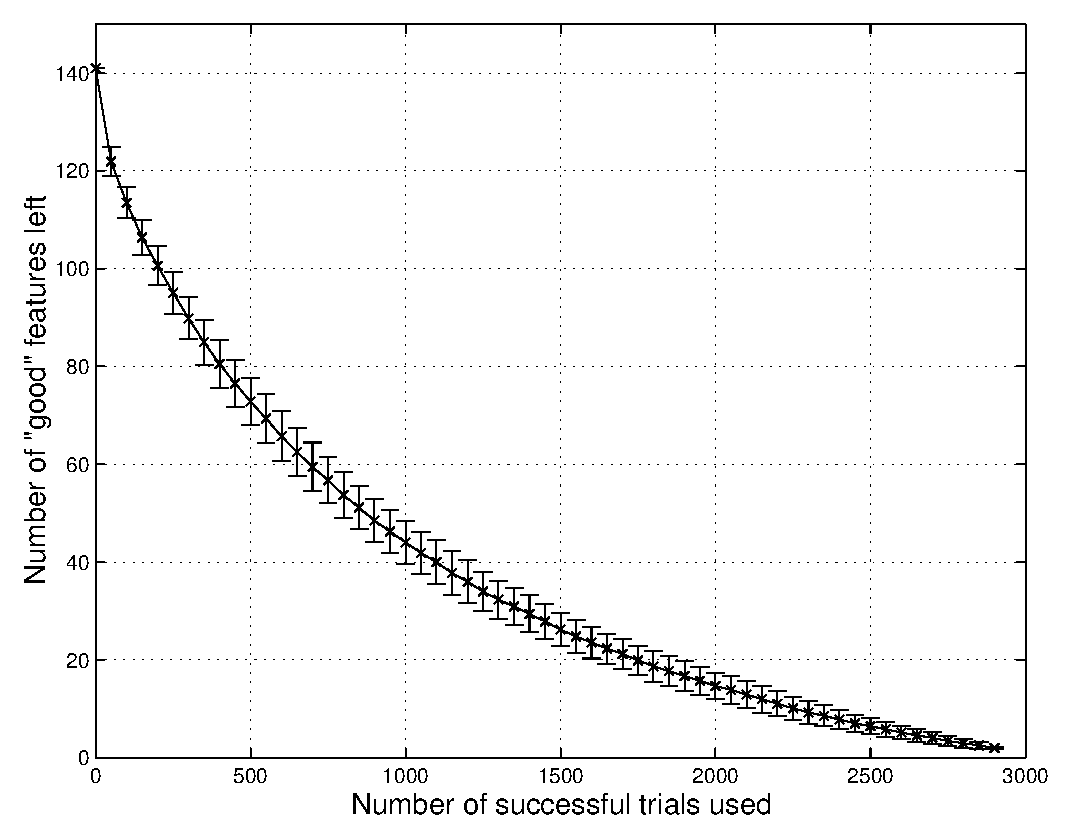
\includegraphics[width=\columnwidth]{applications/ds1000ngood_plot}
  \caption{Progressive \elim{elimination by successful counterexample}
    as successful runs accumulate.  Crosses mark means; error bars
    mark one standard deviation.}
  \label{fig:ngood}
\end{figure}

Figure~\ref{fig:ngood} shows the results.  The crosses mark the mean
number of predicates remaining, while the vertical bars extend one
standard deviation above and below the mean.  The short vertical bars
in this case tells us that there is relatively little diversity in
each of the hundred random subsets at any given size.  The results
show that, on average, 1750 runs are enough to isolate twenty
candidate features, another 500 runs reduces that count by half, and a
total of 2600 runs is enough to narrow the set of good features down
to just five.  One would expect more variety in runs collected from
real users rather than an automated script.  Greater diversity can
only benefit the analysis, as it would provide more novel
counterexamples and therefore may eliminate more uninteresting
predicates more rapidly.

\subsubsection{Performance Impact}

Instrumenting function return values confounds several of the
optimizations proposed in Section~\ref{sec:framework}.  If most
function calls are instrumentation sites, and if most function calls
terminate acyclic regions, then most acyclic regions contain only a
single site and we have poor amortization of sampling overhead.
Furthermore, \texttt{ccrypt} is built one object file at a time, and
we must conservatively assume that any cross-object function call is
not weightless.  Thus, for much of \texttt{ccrypt}, our sampling
transformation devolves to a simpler but slower pattern of checking
the next-sample countdown at each and every site.

%\begin{figure}
%  \centering
%  \small
%  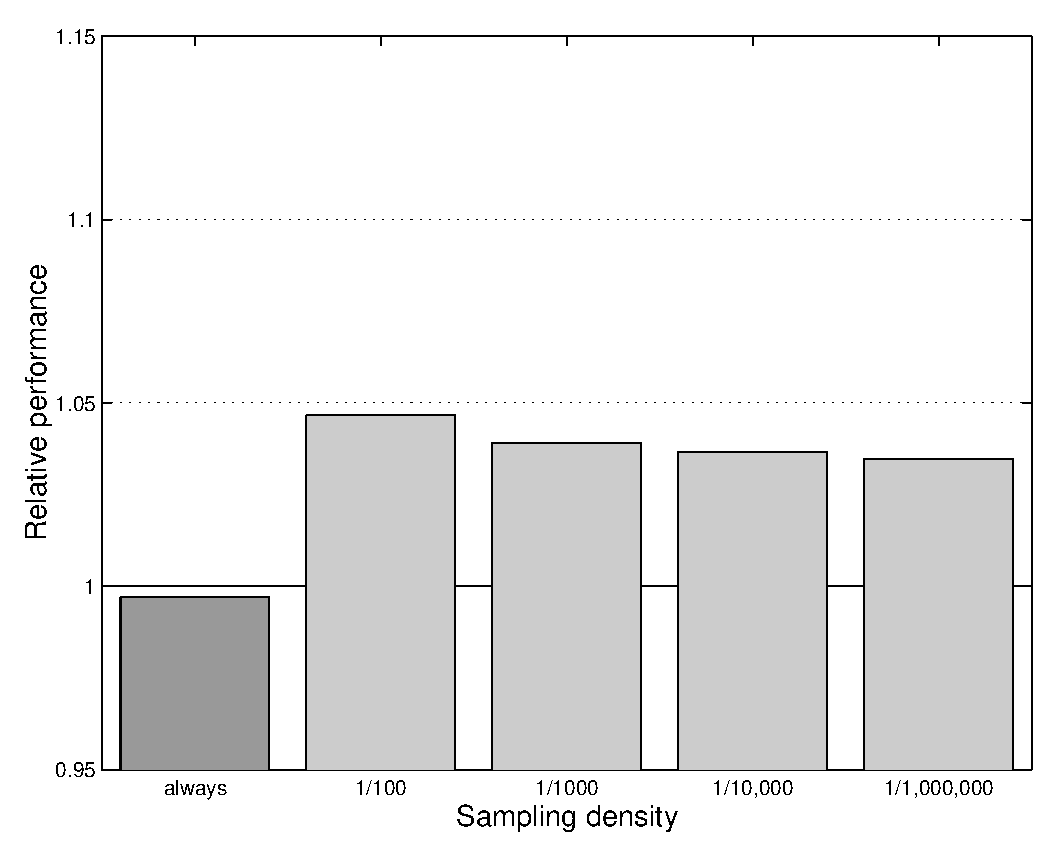
\includegraphics[width=\columnwidth]{applications/ccrypt_density}
%  \caption{Relative performance of \texttt{ccrypt} with unconditional or
%    sampled instrumentation}
%  \label{fig:ccrypt:slowdown}
%\end{figure}

In spite of this, the performance impact of sampled instrumentation is
minimal.  Using an experimental setup similar to that described
earlier in Section~\ref{sec:share:whole}, we find that the overhead
for \nicefrac{1}{1000} sampling is less than 4\%, and progressively
sparser sampling rates shrink this still further.  Unconditional
instrumentation also performs well here, making either reasonable for
this particular application.  In the next section, though, we consider
a more invasive instrumentation strategy that requires sampling to
keep overhead under control.

\subsection{Statistical Debugging}
\label{sec:bc}

In this section we consider the automatic isolation of non-deterministic
bugs.  Recall from Section~\ref{sec:introduction} that a bug is
non-deterministic with respect to a set of program predicates if no predicate
in the set is perfectly correlated with program crashes.  
For this case study we use version 1.06 of the GNU implementation of
\texttt{bc}.  We find that feeding \texttt{bc} nine megabytes of
random input causes it to crash roughly one time in four from, as it
turns out, a previously unknown buffer overrun error.  Since \texttt{bc}
sometimes terminates successfully even when it overruns the buffer,
this bug is non-deterministic.

We instrument \texttt{bc} using a variation on our previous strategy
of counter triples.  We abandon elimination by \elim{successful
counterexample}\footnote{Because the bug is non-deterministic, if we
have enough runs no predicates will satisfy elimination by
\elim{successful counterexample}.} in favor of statistical modeling to
identify behavior that is broadly correlated with failure in spite of
the occasional run that terminates successfully despite triggering the
bug.

\subsubsection{Instrumentation Strategy}

We instrument \texttt{bc} to guess and randomly check a large number
of predicates.  As before, our goal is to identify predicates
that capture bad behavior: false when the program succeeds and true
when the program crashes.  We cast an extremely broad net, but with an
eye toward pointer and buffer errors.  For pointers,
null pointers are of interest.  Relative addresses of pointers
may be interesting as well, as this may capture cases where one
pointer scans within a second pointed-to buffer.  Checking
pointer/pointer equality may reveal aliasing that, when not
anticipated by the programmer, can lead to dangling ``wild'' pointer
bugs.  Scalar variables serve as array indexes, pointer offsets, and
in many other roles; relationships among scalars may reveal buffer
overruns, unanticipated consequences of negative values, invalid
enumeration constants, or a variety of other problems.

At any direct assignment to a scalar variable \texttt{a}, we identify
all other local or global variables $\{ \mathtt{b}_1, \mathtt{b}_2,
\dots, \mathtt{b}_n \}$ that are also in scope and that have the
same type.  We then compare the updated \texttt{a} to each
$\mathtt{b}_i$, and note whether \texttt{a} was less than, equal to,
or greater than $\mathtt{b}_i$.  We compare pointers to same-typed
pointers as well, and additionally compare each pointer for equality
with null.  One comparison between \texttt{a} and $\mathtt{b}_i$,
which bumps one of three counters, is considered to be one
instrumentation site subject to random sampling.  When an instrumented
application terminates, it emits the vector of counter triples along
with a flag indicating whether it completed successfully or was
aborted by a fatal signal.

For \texttt{bc} there are 10,050 counter triples, or 30,150 counters
in all.  The vast majority of these are of no interest: either they
compare completely unrelated variables, or they express relationships
that behave identically in both successful and failed runs.  The
challenge is to find the few predicates that matter.

\subsubsection{Crash Prediction Using Logistic Regression}

To find the important predicates, we recast bug isolation as a
statistical analysis problem.  Each run of \texttt{bc} constitutes one
sample point consisting of 30,150 observed \termdef{features}
(counters) and one binary \termdef{outcome} ($0 = \text{succeeded}, 1
= \text{crashed}$).  Given numerous data points (sampled runs), we
want to identify a subset of our 30,150 features that predict the
outcome.  This is equivalent to the machine learning problem of
learning a binary classifier with feature selection, i.e.,\ using as
few input features as possible.

In the classification setting, we take a set of data with known binary
output (a training set), and attempt to learn a binary classifier that
gives good predictions on a test set.  The learning process usually
involves additional parameters whose values can be determined using a
validation set.  In our case, the end goal is to narrow down the set
of features.  Hence our method must balance good
classification performance with aggressive feature selection.

A binary classifier takes feature values as inputs, and outputs a
prediction of either $0$ or $1$.  \termdef{Logistic regression}
\cite{Hastie01} is a method of learning a binary classifier where the
output function is assumed to be logistic.  The logistic function is a
continuous ``S''-shaped curve approaching 0 on one end, and 1 on the
other.  The output can be interpreted as a probability measure of how
likely the data point falls within class 0 or 1.  Quantizing the
logistic function output then gives us a binary classifier: if the
output is greater than \nicefrac{1}{2}, then the data point is
classified as class 1 (a crash), otherwise it falls under class 0 (a
successful run).  Feature selection can be achieved by
\termdef{regularizing} the function parameters to ignore most input
features, forcing it to form a model that predicts success or failure
using just a small selection of sampled features.  Regularization is
important for our purposes because we expect that most of our features
are wild guesses, but that there may be just a few that correctly
characterize the bug.

While other techniques for combined classification and feature
selection exist, none of them are particularly well-suited for this
problem.  Some methods \cite{Golub:MCC:1999,Tibshirani2002} calculate
a univariate correlation coefficient independently for each feature;
other methods, such as decision trees \cite{00000048}, are more
computationally intensive.  In our dataset, the features are clearly
not independent of each other, and the size of the problem can
potentially be too large for more computationally intensive methods.
Furthermore, logistic regression is a discriminative classification
method, and thus does not make any assumptions about the underlying
distribution of the input.  This is crucial since our features arise
from a decidedly artificial process and would be difficult to
characterize using simple distributions.

Suppose our training set $\mathcal{D}$ consists of $M$ data points
$(x_1,y_1), \ldots, (x_M, y_M) $, where each $x_i \in \Real^N$ denotes
a vector of input predicate counters, and each $y_i = \{0, 1\}$
denotes the corresponding output label.  To learn a good classifier,
we can maximize the \termdef{log likelihood} of the training set.
%%
\begin{equation*}
  \begin{split}
    LL(\mathcal{D}) \:=\:
    \sum_{i=1}^M \, [ & y_i \log P(Y = 1 | x) \\
    + & (1 - y_i) \log (1 - P(Y = 1 | x)) ]
  \end{split}
\end{equation*}

Here the output labels $y_i$ are used as indicator functions to zero
out exactly one of the two terms in each summand.  In logistic
regression, the distribution $P(Y=1|x)$ is modeled as the logistic
function $\mu_{\tilde{\beta}}(x)$ with parameters $\tilde{\beta} = \langle \beta_0 \in
\Real, \beta \in \Real^N \rangle$.
%%
\begin{equation*}
  P(Y = 1 | x) = \mu_{\tilde{\beta}} (x) = \frac{1}{1 + \exp(- \beta_0 - \beta^T x)}
\end{equation*}

The logistic parameters $\beta_0$ and $\beta$ take on the respective roles as
the intercept and slope of the classifier, and essentially weigh the
relative importance of each feature in the final outcome.  We expect
most of the input features to have no influence over the success or
failure of the program, so we place an additional constraint that
forces most of the $\tilde{\beta}$'s toward zero.  This is accomplished by
subtracting a penalty term based on the L1-norm $\norm{\tilde{\beta}}_1 =
\sum_{j=0}^M \abs{\beta_j}$.  We can tune the importance of this
\termdef{regularization term} through a \termdef{regularization
  parameter} $\lambda$.  The penalized log likelihood function is:
%%
\begin{equation*}
  \begin{split}
    LL (\tilde{\beta} | \mathcal{D}, \lambda ) \:=\:
    & \sum_{i=1}^M \, [y_i \log \mu_{\tilde{\beta}} (x_i) + (1 - y_i) \log (1 - \mu_{\tilde{\beta}} (x_i))] \\
    & - \lambda \norm{\beta}_1
  \end{split}
\end{equation*}

An assignment of $\beta$ coefficients that maximizes this function
represents a model that maximizes the fidelity of its predictions
while still limiting itself to form those predictions on the basis of
only a small number of features from the complete feature set.

\subsubsection{Data Collection and Analysis}

Our \texttt{bc} data set consists of 4390 runs with distinct random
inputs and distinct randomized \nicefrac{1}{1000} sampling, of which
2729 are randomly chosen for training, 322 for validation, and 1339
for testing.  Although there are 30,150 raw features, many can be
discarded immediately using \elim{elimination by universal falsehood}:
in the training set 27,242 features are always zero.  Hence the
effective number of features used in training is 2908.  (Elimination
by \elim{lack of failing example} can eliminate another 647 features
that are zero for all failed runs.  However we find that the presence
or absence of these 647 features does not significantly affect the
quality of the regularized logistic regression results.)

To make the magnitude of the $\beta$ parameters comparable, the feature
values must be on the same scale.  Hence all the input features are
shifted and scaled to lie on the interval $[0, 1]$, then normalized to
have unit sample variance.  A suitable value for the regularization
parameter $\lambda$ is determined through validation to be $0.3$.  The model
is then trained using stochastic gradient ascent to reach a local
maximum of the penalized log likelihood.  Using a learning rate of
$10^{-5}$, the model usually converges within sixty iterations through
the training set.  This takes roughly thirty minutes in MATLAB on a
1.8 GHz Pentium 4 CPU with 1 GB of RAM.

Once the model has been trained, predicates with the largest $\beta$
coefficients suggest where to begin looking for the bug.  In our case,
the top five ranked coefficients are well-separated in magnitude from
the rest, and show an unmistakable trend:

\begin{features}
\item storage.c:176: more\_arrays(): indx > scale
\item storage.c:176: more\_arrays(): indx > use\_math
\item storage.c:176: more\_arrays(): indx > opterr
\item storage.c:176: more\_arrays(): indx > next\_func
\item storage.c:176: more\_arrays(): indx > i\_base
\end{features}

\begin{figure}
  \centering
  \VerbatimInput[frame=single,numbers=left,firstnumber=152,fontsize=\scriptsize,xleftmargin=24pt,xrightmargin=12pt]{applications/more_arrays.c}
  \caption{Suspect \texttt{bc} function \texttt{more\_arrays()}.  All
  top-ranked crash-predicting features point to large values of
  \texttt{indx} on line 176.}
  \label{fig:bc:more-arrays}
\end{figure}

The source code for \texttt{more\_arrays()} appears in
Figure~\ref{fig:bc:more-arrays}.  A comment earlier in the same file
suggests that this one of a suite of ``three functions for increasing
the number of functions, variables, or arrays that are needed''.  The
logic is a fairly clear instance of the buffer reallocation idiom,
even to one unfamiliar with the code: line 167 allocates a larger
chunk of memory; line 171 is the top of a loop that copies values over
from the old, smaller array; line 176 completes the resize by zeroing
out the new extra space.  As the comment suggests, there are two
similar functions (\texttt{more\_functions()} and
\texttt{more\_variables()}) nearby that do largely the same thing with
different storage pools.  The text of these three functions is nearly
identical, but each uses different global variables (such as
\texttt{a\_count} versus \texttt{f\_count} versus \texttt{v\_count}).

The top ranked predicates seem bizarre at first glance, because the
variables they relate do not appear to have any real connection to
each other or to \texttt{more\_arrays()}.  For example, \texttt{scale}
tracks significant digits for floating point calculations, while
\texttt{use\_math} records whether an initial math library is to be
loaded.  Why would crashes tend to happen when local variable
\texttt{indx} exceeds these seemingly unrelated globals on this
particular line?  An obvious hypothesis is that \texttt{indx} is
simply unusually large in such cases.  If \texttt{indx} is large, then
it will tend to be larger than any number of otherwise unrelated
variables.  Perhaps crashes occur when the input to \texttt{bc}
defines unusually large numbers of arrays.

Closer scrutiny of \texttt{more\_arrays()} quickly reveals this to be
the case.  The allocation on line 167 requests space for
\texttt{a\_count} items.  The copying loop on line 171 ranges from
\texttt{1} through \texttt{old\_count - 1}.  The zeroing loop on line
176 continues on from \texttt{old\_count} through \texttt{v\_count -
  1}.  And here we find the bug: the new storage buffer has room for
\texttt{a\_count} elements, but the second loop is incorrectly bound
by \texttt{v\_count} instead.  After a quick glimpse at the
neighboring \texttt{more\_variables()} function it is clear that
\texttt{more\_arrays()} was created by copying and pasting
\texttt{more\_variables()} and then changing names like
\texttt{v\_count} and \texttt{v\_names} to \texttt{a\_count} and
\texttt{a\_names}.  The loop bound on line 176 was missed in the
renaming.

The logistic regression model points us at the buggy line, the buggy
variable, and even reveals something of the conditions under which the
bug will appear.  Having found the bug, it is reasonable to ask
whether the statistical analysis could have pointed at it even more
directly.  The mistaken use of \texttt{v\_count} instead of
\texttt{a\_count} on line 176 means that a buffer overrun occurs when
\texttt{indx > a\_count} on line 176.  This does correspond to a
predicate sampled by our system, but this predicate is ranked 240th in
the trained model.  Why was this, the smoking gun, not ranked first?

There are several reasons to consider.  Samples are taken randomly,
while the model itself is trained using stochastic gradient ascent.
Thus, a degree of noise is fundamental to the process.  Even crashing
is not guaranteed: out of 320 runs in which sampling spotted
\texttt{indx > a\_count} at least once, 66 did not crash.  Thus, C
programs can ``get lucky'', meaning that this is not a strict
$\text{overrun} \implies \text{crash}$ implication.  Manual inspection
of the data reveals a high degree of redundancy among many
instrumentation sites within \texttt{more\_arrays()}, meaning that the
model has several features to choose from that have equivalent
predictive power.  This suggests that our counters may be too
fine-grained---we are distinguishing many behaviors that are in
fact so tightly interrelated as to be equivalent.  
%Improving our
%instrumentation scheme and fine-tuning the statistical analysis
%methodology are key areas for continued development.

This bug seems clear enough once found.  However it has been present
and undiscovered at least since 1992 (the time\-stamp on this file in
the oldest version of GNU \texttt{bc} that we can find).  Many bugs
are obvious only once one knows where to look.  The logistic
regression results directed us to one misbehaving variable on one line
of code, out of 8910 lines in \texttt{bc} as a whole.  Our approach
does not automatically find and fix bugs.  But it does suggest where
to start looking, and what sort of scenarios (e.g.\ unusually large
\texttt{indx}) to consider.  Although we are still learning about the
capabilities of this system, and how to interpret its results, we
believe that statistically guided debugging has the potential to make
the process of finding and fixing bugs more efficient.

\subsubsection{Performance Impact}

\begin{figure}
  \centering
  \small
  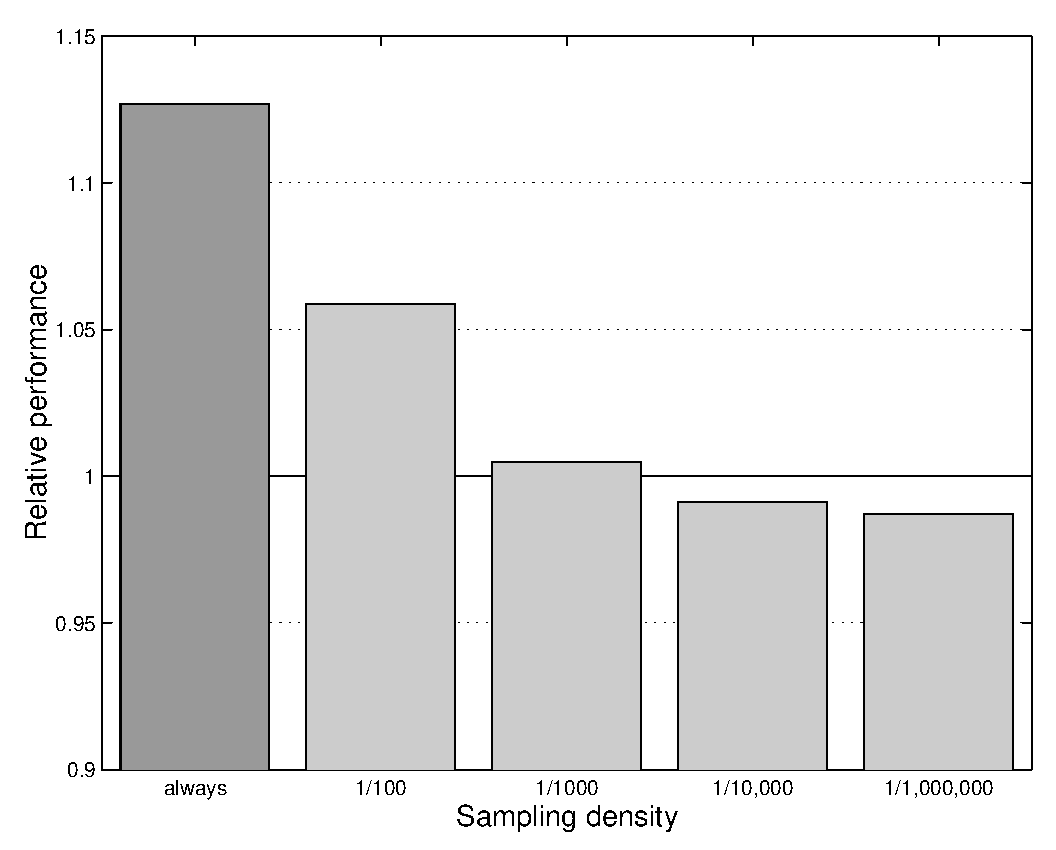
\includegraphics[width=\columnwidth]{applications/bc_density}
  \caption{Relative performance of \texttt{bc} with unconditional or
    sampled instrumentation}
  \label{fig:bc:slowdown}
\end{figure}

Our \texttt{bc} instrumentation is quite dense.  The leftmost bar in
Figure~\ref{fig:bc:slowdown} shows that if this instrumentation is
added without sampling, the performance penalty is correspondingly
large: 13\%.  A sampling density of \nicefrac{1}{100} cuts this in
half (6\%).  At the \nicefrac{1}{1000} density used in our statistical
debugging experiment, the penalty is barely measurable (0.5\%).  Still
lower densities show small, unexpected speedups relative to
uninstrumented code.  This is apparently due to effects such as
changes in relative code alignment, cache behavior, measurement noise,
and other unpredictable factors.  
%Thus, we achieved an important goal:
%we can sample program behavior at densities that allow us to isolate
%real bugs while imposing an overhead on clients that is so small as to
%be unmeasurable in practice.


%% LocalWords: DNDEBUG SPECINT rrr rrrr pre ijpeg treeadd li ccrypt
%% LocalWords: xreadline bc malloc indx opterr func firstnumber
%% LocalWords: fontsize xleftmargin xrightmargin

\section{Related Work}
\label{sec:related-work}

Sampling has a long history, with most applications focusing on
performance profiling and optimization.  Any sampling system must
define a trigger mechanism that signals when a sample is to be taken.
Typical triggers include periodic hardware timers/interrupts
\cite{Burrows:2000:EFV,Traub:200:EILPP,Whaley:337483}, periodic
software event counters (e.g.  every $n$th function call)
\cite{Arnold:2000:ACCTS}, or both.  In most cases, the sampling
interval is strictly periodic; this may suffice when hunting for large
performance bottlenecks, but may systematically miss rare events.

The Digital Continuous Profiling Infrastructure
\cite{Anderson:1997:CPW} is unusual in choosing sampling intervals 
randomly.  However, the random distribution is uniform, such as one
sample every 60K to 64K cycles.  Samples thus extracted are not
statistically fair in the sense of a Bernoulli process.
If one sample is taken, there is zero chance of taking any sample in
the next 1--59,999 cycles and zero chance of
\emph{not} taking exactly one sample in the next 60K--64K cycles.  We
trigger samples based on a geometric distribution, which correctly
models the interval between independent coin tosses.  The resulting
data is a statistically rigorous fair random sample, which in turn
grants access to a large domain of powerful statistical analyses.

Recent work in trace collection has focused on program understanding.
Techniques for capturing program traces confront challenges similar to
those we face here, such as minimizing performance overhead and
managing large quantities of captured data.  Dynamic analysis in
particular must encode, compress, or otherwise reduce an incoming
trace stream in real time, as the program runs
\cite{Demsky:RBEOOP:2002,ICSE01*221}.  It may be difficult to directly
adapt dynamic trace analysis techniques to a domain where the trace is
sampled and therefore incomplete.  
%However, it may be possible to
%combine these approaches so that one fairly and randomly samples short
%trace ``bursts'', with complete data collection within each burst.
%This would allow us to examine sequences of interrelated events, a
%task which is difficult under our current, strictly Bernoullian
%regime.

Our effort to understand and debug programs by selecting predicates is
partly inspired by Daikon \cite{ernst2001}.  Like Daikon, we begin
with fairly unstructured guesses and eliminate those which do not
appear to hold.  Daikon collects a complete trace of individual
program values; generation and testing of possible invariants occurs
off line.  This gives Daikon greater flexibility to consider a
larger family of candidate invariants then we have examined, as a
significant part of our predicate testing happens within the client
itself.  With a large enough user population, though, the myriad
invariants considered by Daikon could certainly be tested.

The DIDUCE project \cite{Hangal:DIDUCE:2002} also attempts to identify
program invariants.  Unlike Daikon, most processing does take place
within the client program.  As in our study, DIDUCE attempts to relate
changes in predicates to the manifestation of bugs.  However, DIDUCE
performs complete tracing and focuses on discrete state changes, such
as the first time a predicate transitioned from true to false.  Our
approach is more probabilistic: we wish to identify broad trends over
time that correlate predicate violations with increased likelihood of
failure.  
%Our approach explicitly accommodates the possibility of
%``getting lucky'', such as overrunning a buffer but not actually
%crashing.  DIDUCE works in the context of a safe language (Java) in
%which most forms of getting lucky cannot happen.


% LocalWords:  DIDUCE

\section{Privacy and Security}
\label{sec:privsec}

\aside{Remember to discuss database poisoning by malicious or selfish clients}

\aside{Non-interference, taint analysis, etc.}

\section{Conclusions}
\label{sec:conclusions}

We have described a sampling infrastructure for gathering information about
software from the set of runs produced by its user community.  To ensure
that rare events are accurately represented, we use a Bernoulli process to do the sampling,
and we have described an efficient implementation of that process.
We have also presented two sample applications: sharing the overhead of assertions, and 
using logistic regression of a large number of sampled runs to help isolate
the location of a bug.


\bibliography{acm-dlp,agent,all,ec00,icse01,jamstatassoc,lloyd,personal,pnas,popl02,refs,security,SEL-HPC,SEPL-subset,sigplan2000,tocs}

\end{document}


%% LocalWords: acm dlp ec jamstatassoc popl SEPL sigplan tocs icse lloyd pnas
%% LocalWords:  SEL HPC privsec


%% LocalWords:  abbrv acm proc sp sig mailto EIA CCR ACI LLNL
